\chapter{Phases of Matter}

You have experienced $H_2O$ in three phases of matter:
\begin{itemize}
\item Ice is $H_2O$ in the solid phase.  At standard pressure,  when the temperature of $H_2O$ is below $0^\circ$ C,  it is a solid.  
\item Water is $H_2O$ in the liquid phase.  At standard pressure, when the temperature of $H_2O$ is between $0^\circ$ C and  $100^\circ$ C,  it is a liquid.
\item Water vapor (or steam) is the gas phase.  At standard pressure,  when the temperature of $H_20$ is above $100^\circ$ C,  it is a gas.
\end{itemize}

Let's look at some of the properties of the three phases:

\begin{tabular}{p{5cm}|p{5cm}|p{5cm}}
Gas & Liquid & Solid \\
\hline
Assumes the volume and shape of its container & 
Assumes the shape, but not the volume, of its container &
Retains its shape and volume \\
\hline
Compressible & Not compressible & Not compressible \\
\end{tabular}

\section{Thinking Microscopically About Phase}

As mentioned in an early chapter,  there are intermolecular forces that attract molecules to each
other. A pair of molecules will have very strong intermolecular forces or very weak intermolecular forces,
depending on what atoms they are made of.

For example,  two helium molecules are very weakly attracted to each other due to weak intermolecular forces.   Two molecules of $NaCl$ (table salt) will experience very strong intermolecular attraction.

In a gas,  the molecules have lots of room to roam and lots of kinetic energy: The intermolecular attraction has very little effect.

In a liquid,  the molecules are sticking close together,  but are still moving around,  sort of like bees in a hive.

In a solid, the molecules are not changing their configuration, and the kinetic energy they have is just expressed as vibrations within that configuration. You can imagine them like eggs vibrating in a carton.

As you would expect, molecules with strong intermolecular attraction require more kinetic energy to change phases.  For example, helium is a liquid below $-269\circ$ C.  $NaCl$, on the other hand, is a liquid between $801^\circ$ and $1,413^\circ$ C.  

The temperatures I just gave you are at standard pressure (100 kPa or 1 atm).  Pressure also has a role in phase change.  In low pressure environments,  it is much easier for the molecules to make the jump to being a gas.

For example,  if you climb a mountain until the atmospheric pressure is 70 kPa,  your water will boil at about $90^\circ$ C.  

If you rise in a balloon until the atmospheric pressure is 500 Pa,  if your water is colder than $-2^\circ$ C,  it will be ice.  If it is warmer it will vaporize.    There is no liquid water at 500 Pa!

For any molecule,  we could observe its phase at a wide range of temperatures and pressures.  This would let us create a phase diagram.  Here is the phase diagram for $H_2O$:

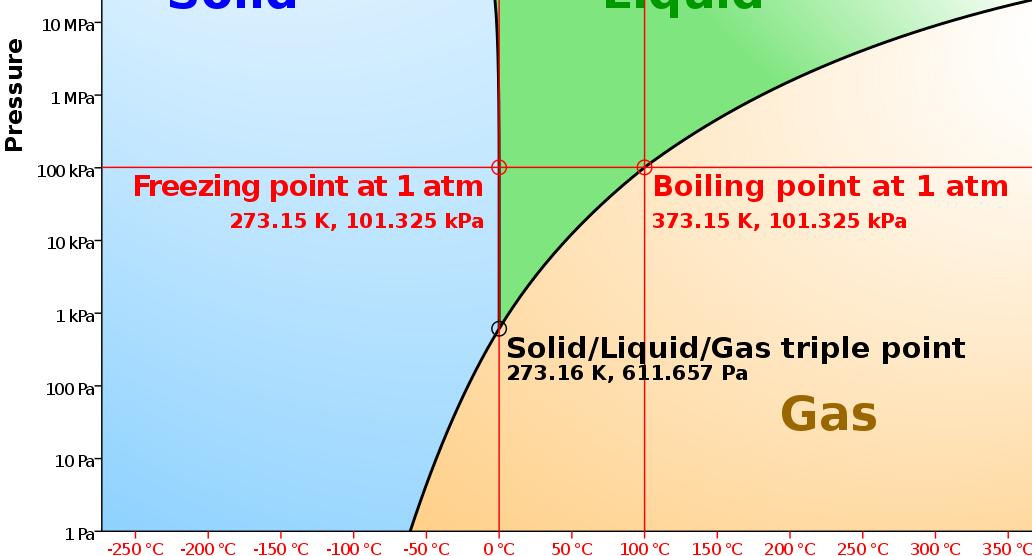
\includegraphics[width=\textwidth]{waterphase_edit.png}

(FIXME: This diagram needs to be recreated prettier.)

\section{Phase Changes and Energy}

The molar heat capacity of ice is about 37.7 J/mol-K.  That is, it takes about 37.7 Joules of energy to raise the temperature of one mole of ice by one degree kelvin.

The molar heat capacity of liquid water is about 75.4 J/mol-K.  For water vapor, it is about 36.6 J/mol-K.

Imagine you have mole of ice at $173^\circ$ K, and you are going to gradually add kinetic energy into it until you have steam at $473^\circ$ K.  You might guess (incorrectly) that the temperature vs. energy applied would look like this:

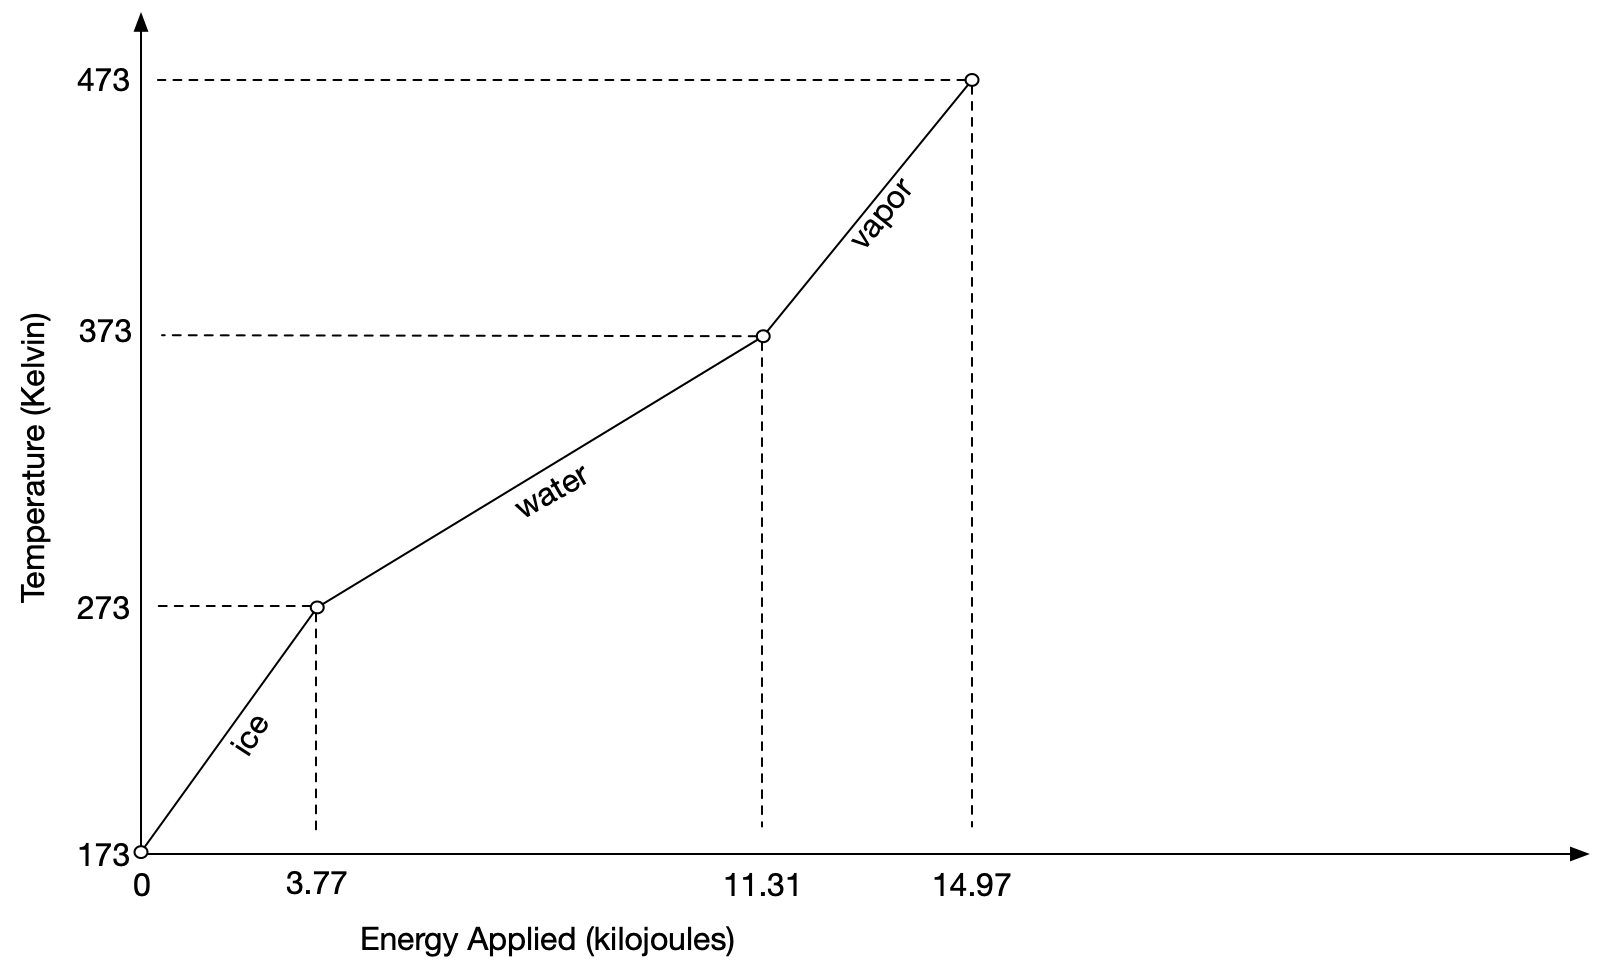
\includegraphics[width=0.8\linewidth]{energynaive.png}

However,  once molecules are nestled into their solid state (like eggs in cartons),  it take extra energy to make them move like a liquid.  How much more energy?  For water,  it is 6.01 kilojoules per mole.  This is known as \newterm{the latent heat of melting} or \newterm{the heat of fusion}.

Similarly,  the transition from liquid to gas takes energy.  At standard pressure,  converting a mole of liquid water to vapor requires 40. 7 kilojoules per mole.  This is known as \newterm{the latent heat of vaporization}. So, the graph would actually look like this:

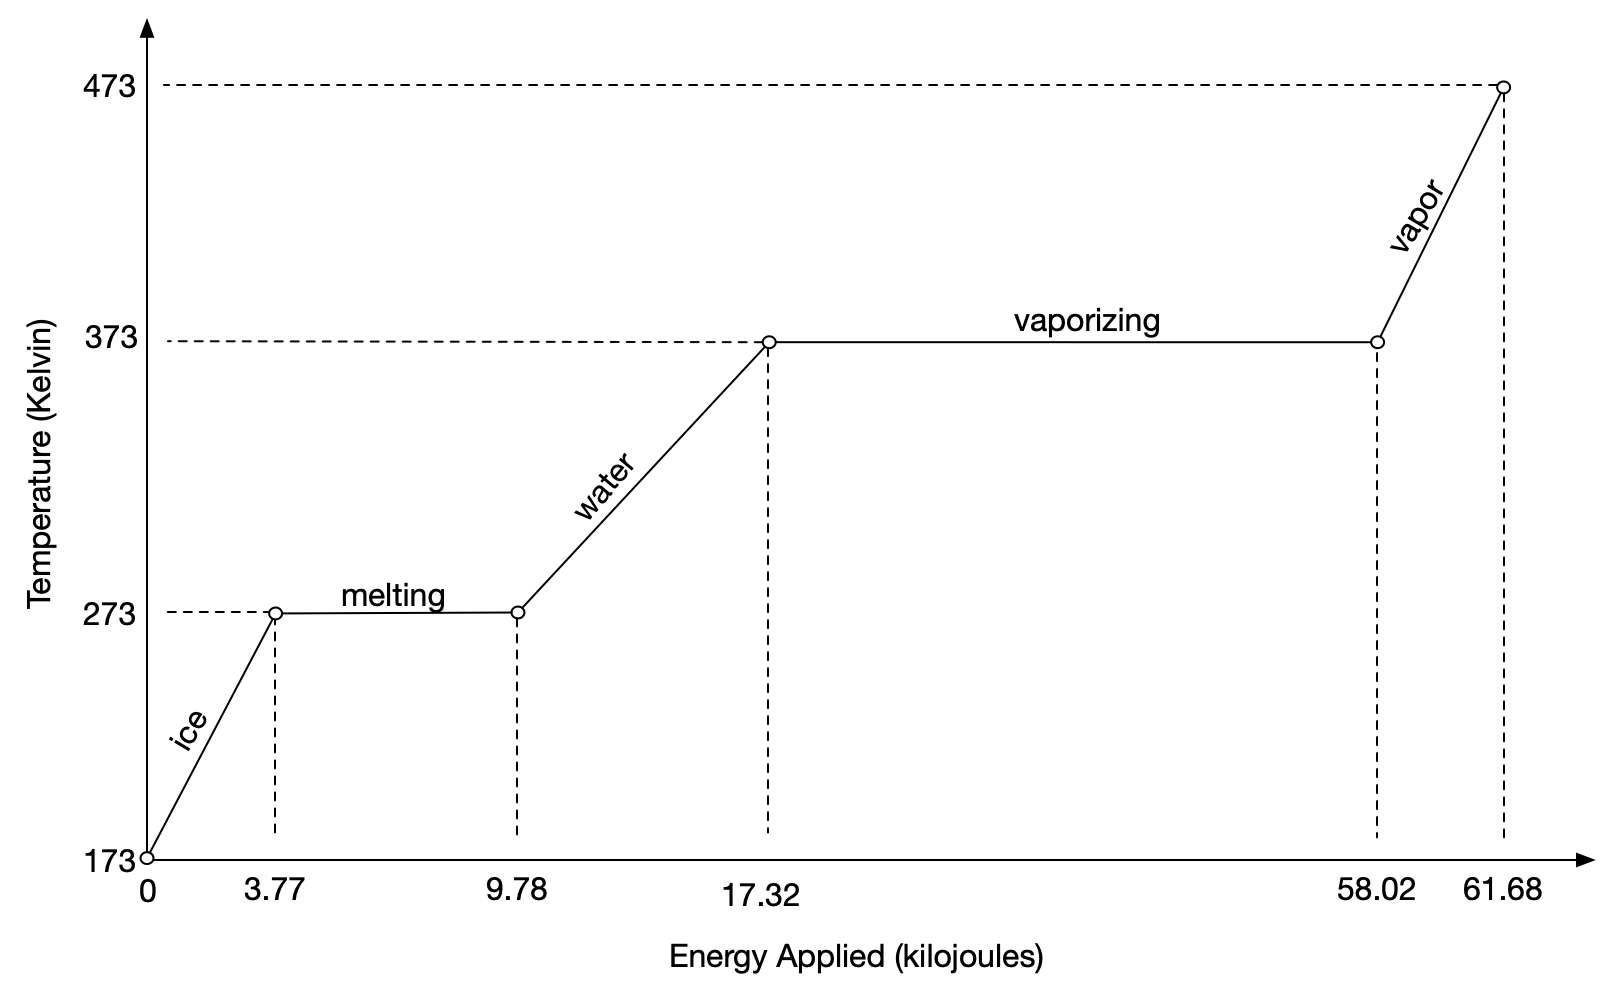
\includegraphics[width=0.8\linewidth]{energysoph.png}

Note that just as melting and vaporizing require energy, going the other way (freezing and condensing, respectively) give off energy.  Thus, we can store energy using the phase change.

\section{How a Rice Cooker Works}

A rice cooker is a bowl with a lid and an electric heating element.  You put rice and water into the bowl and turn on the heating element.   The heating element pushes kinetic energy into the water, which gets warmer and eventually starts to boil.

How does the rice cooker know when to turn off (or at least down to a low-heat "keep warm" mode) before the rice starts to burn?

As long  as there is a little liquid water in the bottom of the bowl, the rice won't burn, so the question is really "How does it know when there is no more liquid water in the bottom of the bowl?"

There is a mechanism (and there have been a few different versions of this mechanism)  that monitors the temperature of the surface of the bowl.  As long as there is liquid water in the bowl,  it \emph{cannot} go above $100^\circ$ C!  When all the water has been absorbed by the rice or turned to steam,  the temperature rises above $100^\circ$ C, and the mechanism cuts off the heat.

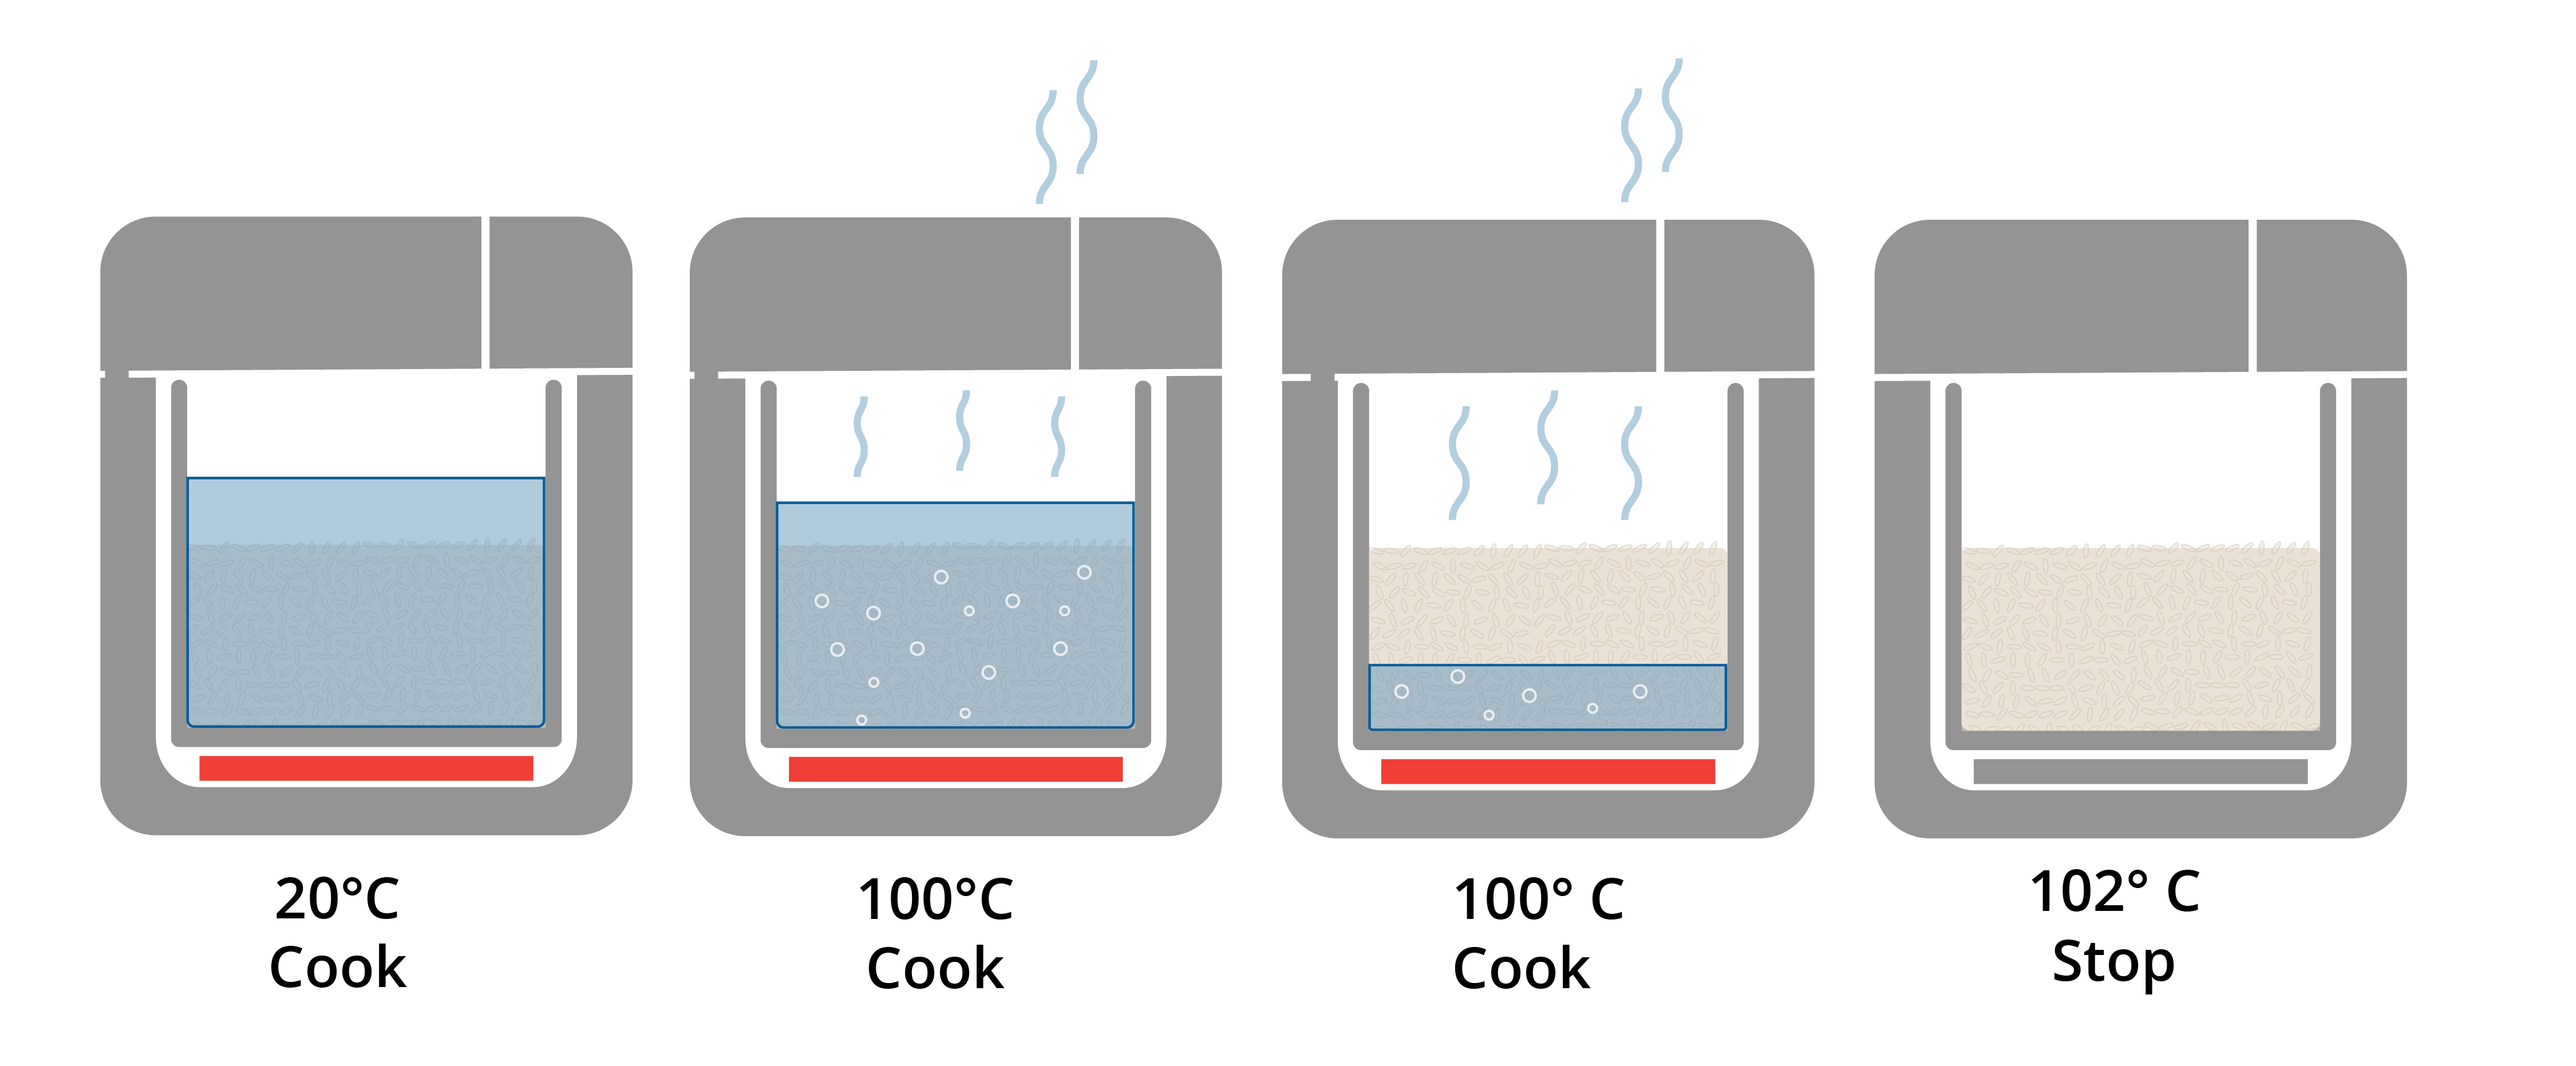
\includegraphics[width=0.9\linewidth]{riceCookerPhase.png}

\begin{Exercise}[title={Using Water For Thermal Energy Storage}, label=waterthermal]
Tom is building a passive solar house; the front of his house is a greenhouse.  He also likes to 
eat dinner in the greenhouse.  He will have barrels (painted black) that hold 159 liters of water.  His plan is to let the sun heat the barrels to $33^\circ$ C by the time the sun goes down.  (Any warmer and it would be unpleasant to eat dinner near them.)

At night, he will circulate air past the barrels and through his house.  He is OK with the house and the barrels dropping to $17^\circ$ C.

Looking at the insulation on his house and the expected nighttime temperatures,  Tom estimates that he needs to store 300,000 kJ of energy in the barrels.

A mole of water is about 0.018 liters.

The molar heat capacity of water is about 75.38 J/mole-K.

How many barrels of water does Tom need to install in his greenhouse?

\end{Exercise}
\begin{Answer}[ref=waterthermal] 

When one mole of water goes from $33^\circ$ to $17^\circ$,  it will give off $(75.38)(33-17) = 1,206$ Joules or $1.206$ kJ. 

Tom needs 300,000 kJ,  so he needs $300,000/1.206 =   248,739.72$ moles of water.

How many liters is that?  $248,739.72 * 0.018 = 4,477.31$ liters.

How many barrels is that? $4,477.31 / 159 = 28.16$ barrels.  He will need 29 barrels.
  
\end{Answer}


\begin{Exercise}[title={Using Mirabilite For Thermal Energy Storage}, label=mirabilite]

Water barrels are going to take up too much of Tom's greenhouse!

There is a substance known as mirabilite, or Glauber's salt,  or sodium sulfate decahydrate.  It is relatively cheap to produce, and it has a melting point of $32.4^\circ$ C.

The molar heat capacity of mirabilite is 550 J/mole-K.

The latent heat of melting mirabilite is 82 kJ per mole.

Mirabilite comes in a powder form.  Assume that a mole of mirabilite occupies about 0.22 liters.

If Tom fills his barrels with mirabilite,  how many barrels will he need?

\end{Exercise}
\begin{Answer}[ref=mirabilite] 

When one mole of mirabilite goes from $33^\circ$ to $17^\circ$,  it will give off $(550)(33-17) + 82,000 = 90,800$ Joules or $90.8$ kJ. 

Tom needs 300,000 kJ,  so he needs $300,000/90.8 =   3,304$ moles of mirabilite.

How many liters is that?  $3,304 * 0.22 = 726.9$ liters.

How many barrels is that? $726.9 / 159 = 4.57$.  He will need 5 barrels.
  
\end{Answer}

\section{Thinking Statistically About Phase Change}

We like to say simple things like "At $100^\circ$ C,  water changes to vapor." However,  remember what
temperature is: Temperature tells you how much average kinetic energy the water molecules have.   The key word here is \emph{average}; Some molecules are going faster than average and some are going slower.

A puddle in the street on a warm night will evaporate. It isn't  $100^\circ$ C.  Why would the puddle turn to vapor?

While the \emph{average} molecule in the puddle doesn't have enough energy to escape the intermolecular forces,  some of the molecules do.  When a molecule on the surface has enough velocity (toward the sky!) to escape the intermolecular forces,  it becomes vapor and leaves the puddle.

What happens to the temperature of the puddle during this sort of evaporation?  Temperature is proportional to the average kinetic energy of the molecules.  If a bunch of molecules with a lot of kinetic energy leave,  the average kinetic energy (of the molecules that remain) will decrease.

The most obvious example of this process is sweating:  When your body is in danger of getting too hot,  sweat comes out of your pores and covers your body.   The fastest moving molecules escape your body,  taking the excess kinetic energy with them.

\subsection{Evaporative Cooling Systems}

An evaporative cooling system (also called a "Swamp Cooler") uses this idea to cool air.  You can imagine a fan drawing warm air through a duct from the outside.   Before the air is released inside,  it passes very close to a cloth that is soaked with water.   The warm air molecules (which has a lot of kinetic energy) slam into the water molecules,  some of which get enough kinetic energy to become vapor.  The cool air and the water vapor then enter the room.

"Wait, wait, wait," you say, "The heat hasn't gone away.  It is just transferred into the water molecules."

Remember that it takes 40.7 kilojoules to change a mole of liquid water at $100^\circ$ C to water vapor at $100^\circ$.  Escaping those intermolecular bonds takes a great deal of energy!

Thus, if a mole of water evaporates,   it is because it has absorbed 40.7 kj of heat you can feel
 (\newterm{sensible heat}) and used it to liberate the molecules from their intermolecular bonds.  For
 convenience,  physicists call this \newterm{latent heat}.
 
 \subsection{Humidity and Condensation}
 
When a puddle is evaporating on a warm day,  there might be some water vapor already in the air.  Even as the water molecules in the puddle are evaporating,  some water molecules in the air are crashing into the puddle and become liquid again.  (We say they \newterm{condensed},  thus the word \newterm{condensation} to describe the water that accumulates on a cold glass on a warm day.)
 
When there is a lot of water vapor in the air,  the puddle will evaporate more slowly.   In fact,  if there is enough
water vapor in the air,  the puddle won't evaporate at all.   At this point,  we say "The relative humidity is 100\%."   That is, relative to the amount of water the air will hold,  it already has 100\% that amount.

Neither sweating nor evaporative cooling systems work well when the relative humidity is high.

As the temperature goes up,  the air can hold more water.  We usually notice it when it goes the other way: the air cools and has more water vapor than it can hold.  Some of the water vapor condenses into water droplets.  If the droplets land on something,  we call it "dew".  If it is high in the sky,  we call the droplets "a cloud".  If it is near the ground,  we call it "fog".



 